\documentclass[11pt,letterpaper]{article}

% ── Packages ──────────────────────────────────────────────────
\usepackage[margin=1in]{geometry}
\usepackage{amsmath,amssymb}
\usepackage{booktabs}
\usepackage{graphicx}
\usepackage{xcolor}
\usepackage{hyperref}
\usepackage{enumitem}
\usepackage{tikz}
\usepackage{tcolorbox}
\usepackage{fancyhdr}
\usepackage{tabularx}
\usepackage{multirow}
\usepackage{colortbl}
\usepackage{pgfgantt}
\usepackage{listings}

\tcbuselibrary{listings,skins,breakable}
\usetikzlibrary{arrows.meta,positioning,shapes.geometric,calc}

% ── Colors ────────────────────────────────────────────────────
\definecolor{zetablue}{RGB}{30,70,130}
\definecolor{phase1}{RGB}{41,128,185}
\definecolor{phase2}{RGB}{39,174,96}
\definecolor{phase3}{RGB}{192,57,43}
\definecolor{phase4}{RGB}{142,68,173}
\definecolor{milestone}{RGB}{243,156,18}
\definecolor{codebg}{RGB}{248,248,248}
\definecolor{codeborder}{RGB}{200,200,200}
\definecolor{notebg}{RGB}{240,248,255}
\definecolor{warnbg}{RGB}{255,245,238}
\definecolor{warnred}{RGB}{180,30,30}
\definecolor{successbg}{RGB}{240,255,240}
\definecolor{successgreen}{RGB}{30,130,50}
\definecolor{lightgray}{RGB}{245,245,245}
\definecolor{keywordblue}{RGB}{0,0,180}
\definecolor{commentgreen}{RGB}{0,128,0}

% ── Hyperref ──────────────────────────────────────────────────
\hypersetup{
    colorlinks=true,
    linkcolor=zetablue,
    citecolor=zetablue,
    urlcolor=zetablue,
}

% ── Code listings ─────────────────────────────────────────────
\lstdefinestyle{cudastyle}{
    language=C++,
    basicstyle=\ttfamily\footnotesize,
    keywordstyle=\color{keywordblue}\bfseries,
    commentstyle=\color{commentgreen}\itshape,
    backgroundcolor=\color{codebg},
    frame=single,
    rulecolor=\color{codeborder},
    numbers=left,
    numberstyle=\tiny\color{gray},
    numbersep=6pt,
    tabsize=4,
    showstringspaces=false,
    breaklines=true,
    xleftmargin=2em,
    framexleftmargin=1.5em,
    morekeywords={__global__,__device__,__shared__,__constant__,__ldg,
                  dim3,cudaMalloc,cudaFree,cudaMemcpy,cudaMemcpyToSymbol,
                  cudaMemPrefetchAsync,cudaMallocManaged,
                  cudaDeviceSynchronize,blockIdx,blockDim,threadIdx},
}

\lstdefinestyle{bashstyle}{
    language=bash,
    basicstyle=\ttfamily\footnotesize,
    backgroundcolor=\color{codebg},
    frame=single,
    rulecolor=\color{codeborder},
    showstringspaces=false,
    breaklines=true,
    xleftmargin=1em,
    framexleftmargin=0.5em,
}

% ── Header/Footer ─────────────────────────────────────────────
\pagestyle{fancy}
\fancyhf{}
\fancyhead[L]{\small\textcolor{zetablue}{\textbf{Zetascope}} --- GPU Engineering Plan}
\fancyhead[R]{\small\textcolor{gray}{Internal --- Confidential}}
\fancyfoot[C]{\small\thepage}
\renewcommand{\headrulewidth}{0.4pt}

% ── Custom boxes ──────────────────────────────────────────────
\newtcolorbox{notebox}[1][]{
    colback=notebg, colframe=zetablue,
    fonttitle=\bfseries, title={#1},
    arc=2pt, boxrule=0.5pt,
    left=8pt, right=8pt, top=4pt, bottom=4pt,
}

\newtcolorbox{warnbox}[1][]{
    colback=warnbg, colframe=warnred,
    fonttitle=\bfseries\color{warnred}, title={#1},
    arc=2pt, boxrule=0.5pt,
    left=8pt, right=8pt, top=4pt, bottom=4pt,
}

\newtcolorbox{successbox}[1][]{
    colback=successbg, colframe=successgreen,
    fonttitle=\bfseries\color{successgreen}, title={#1},
    arc=2pt, boxrule=0.5pt,
    left=8pt, right=8pt, top=4pt, bottom=4pt,
}

\newtcolorbox{milestonebox}[1][]{
    colback=milestone!10, colframe=milestone,
    fonttitle=\bfseries\color{milestone!80!black}, title={#1},
    arc=2pt, boxrule=0.5pt,
    left=8pt, right=8pt, top=4pt, bottom=4pt,
}

% ── Title ─────────────────────────────────────────────────────
\title{%
    \vspace{-1cm}
    {\Large\textcolor{zetablue}{\textbf{Zetascope, Inc.}}}\\[0.3cm]
    {\LARGE NVIDIA Orin GPU Engineering Plan}\\[0.2cm]
    {\Large 8-Week Onboarding and Optimization Roadmap\\
    for Track-Before-Detect Flight Software}\\[0.3cm]
    \rule{\textwidth}{0.4pt}
}
\author{}
\date{\today}

% ==============================================================
\begin{document}
\maketitle
\thispagestyle{fancy}

\tableofcontents
\newpage

% ==============================================================
\section{Executive Summary}
% ==============================================================

This document defines the 8-week engineering plan for a senior GPU
engineer joining Zetascope to port and optimize the Track-Before-Detect
(TBD) algorithm from development hardware (NVIDIA RTX-class desktop GPUs)
to the NVIDIA Jetson AGX Orin platform. The Orin deployment is a
\textbf{DARPA program requirement} for the TBD2 contract: all delivered
code must execute on Orin or equivalent hardware.

The plan is structured in four phases:
\begin{enumerate}[leftmargin=2em]
    \item \textbf{Weeks 1--2:} Platform bring-up, baseline port, and profiling
    \item \textbf{Weeks 3--4:} Memory system optimization for unified memory
    \item \textbf{Weeks 5--6:} Kernel optimization and compute tuning
    \item \textbf{Weeks 7--8:} Pipeline integration and flight-mode validation
\end{enumerate}

Each phase concludes with a concrete milestone deliverable. The engineer
will work from an existing, validated CUDA codebase running on RTX
hardware; the algorithmic correctness is already established.

% ==============================================================
\section{Hardware Context}
\label{sec:hardware}
% ==============================================================

\subsection{NVIDIA Jetson AGX Orin Specifications}

\begin{table}[h]
\centering
\caption{Orin AGX vs.\ RTX 4090 comparison.}
\label{tab:hw_compare}
\begin{tabular}{@{}lrrl@{}}
\toprule
\textbf{Parameter} & \textbf{Orin AGX 64GB} & \textbf{RTX 4090} & \textbf{Ratio} \\
\midrule
Architecture         & Ampere (SM 8.7)   & Ada Lovelace (SM 8.9) & --- \\
CUDA cores           & 2,048             & 16,384          & $0.125\times$ \\
GPU clock (max)      & 1.3\,GHz          & 2.52\,GHz       & $0.52\times$ \\
FP32 throughput      & 5.3\,TFLOPS       & 82.6\,TFLOPS    & $0.064\times$ \\
Memory               & 64\,GB unified    & 24\,GB GDDR6X   & $2.7\times$ capacity \\
Memory bandwidth     & 204.8\,GB/s       & 1,008\,GB/s     & $0.20\times$ \\
L2 cache             & 4\,MB             & 96\,MB          & $0.042\times$ \\
TDP                  & 15--60\,W         & 450\,W          & $0.033$--$0.13\times$ \\
\bottomrule
\end{tabular}
\end{table}

\subsection{Key Architectural Differences}

The performance gap is significant, but three architectural differences
dominate the optimization strategy:

\begin{enumerate}[leftmargin=2em]
    \item \textbf{Unified memory.} The Orin shares a single physical memory
    between CPU and GPU. There is no PCIe transfer; instead, the GPU
    accesses memory directly. However, memory pages must be \emph{resident}
    on the GPU-accessible fabric for full bandwidth. Unmanaged access
    patterns cause page faults and catastrophic slowdowns.

    \item \textbf{L2 cache (4\,MB vs.\ 96\,MB).} On the RTX 4090, the
    entire frame dataset for the interview problem (4\,MB) fits in L2.
    On Orin, \emph{nothing} fits in L2 at operational scale. Every
    optimization that reduces L2 working set or improves temporal locality
    has outsized impact on Orin.

    \item \textbf{Thermal throttling.} The Orin operates under a strict
    thermal envelope. Sustained full-load kernels will hit thermal limits
    and clock down. Kernel design must consider sustained throughput, not
    just peak burst performance.
\end{enumerate}

\begin{warnbox}[Critical Constraint]
Optimization intuitions from desktop GPUs do not transfer directly to
Orin. Profile on actual Orin hardware early and often. Desktop profiling
is necessary but not sufficient.
\end{warnbox}

% ==============================================================
\section{Prerequisites and Inputs}
\label{sec:prerequisites}
% ==============================================================

The engineer will receive the following on Day 1:

\begin{table}[h]
\centering
\caption{Inputs provided to the GPU engineer.}
\begin{tabular}{@{}p{4.5cm}p{9cm}@{}}
\toprule
\textbf{Item} & \textbf{Description} \\
\midrule
\texttt{tbd\_problem.py} &
    Python reference implementation with data generator, brute-force
    algorithm, and NumPy-vectorized solver. Defines the algorithm spec
    and generates validation datasets. \\
\addlinespace
\texttt{tbd\_solution.cu} &
    Interview-scale CUDA reference ($256 \times 256$, 16 frames, 625
    velocities). Validated correct on RTX hardware. \\
\addlinespace
\texttt{tbd\_fullscale.cu} &
    Full-scale benchmark ($4000 \times 2500$, 300 frames, $\sim$20K
    velocities). Self-contained data generation on GPU. \\
\addlinespace
Algorithm specification &
    Mathematical description of the shift-and-stack test statistic,
    velocity grid construction, boundary handling, and detection
    criterion (Sections~2--3 of the interview document). \\
\addlinespace
Orin developer kit &
    Jetson AGX Orin 64\,GB with JetPack SDK installed, accessible via
    SSH. Provided by Aethero partnership. \\
\addlinespace
Validation datasets &
    Synthetic datasets with known ground truth at multiple difficulty
    levels (varying SNR, image size, velocity range). Generated by
    \texttt{tbd\_problem.py} with configurable parameters. \\
\bottomrule
\end{tabular}
\end{table}

% ==============================================================
\section{Phase 1: Platform Bring-Up and Baseline (Weeks 1--2)}
\label{sec:phase1}
% ==============================================================

\subsection{Objectives}

\begin{enumerate}[leftmargin=2em]
    \item Get the existing CUDA code compiling and running on Orin
    \item Establish baseline performance numbers
    \item Identify the dominant bottlenecks via profiling
    \item Understand the gap between Orin and RTX performance
\end{enumerate}

\subsection{Week 1: Cross-Compilation and Initial Port}

\subsubsection{Day 1--2: Environment setup}

\begin{itemize}[leftmargin=2em]
    \item Install JetPack 6.x SDK on the Orin developer kit (if not
    pre-installed by Aethero). Verify CUDA 12.x toolkit, cuDNN, and
    Nsight Systems/Compute are available.
    \item Set up the build toolchain. The primary change is the target
    architecture flag:

\begin{lstlisting}[style=bashstyle]
# RTX 4090 (Ada Lovelace)
nvcc -O3 -arch=sm_89 --use_fast_math -o tbd_solution tbd_solution.cu

# Orin (Ampere)
nvcc -O3 -arch=sm_87 --use_fast_math -o tbd_solution tbd_solution.cu
\end{lstlisting}

    \item Verify that \texttt{tbd\_solution.cu} (interview-scale) compiles
    and produces the correct detection result on Orin. This should require
    zero code changes beyond the architecture flag.

    \item Record baseline timing:
    \begin{itemize}
        \item Interview-scale: expected $\sim$50--200\,ms on Orin
            (vs.\ $\sim$10--30\,ms on RTX 4090)
        \item Note: this is a sanity check, not a performance target
    \end{itemize}
\end{itemize}

\subsubsection{Day 3--4: Full-scale benchmark on Orin}

\begin{itemize}[leftmargin=2em]
    \item Compile and run \texttt{tbd\_fullscale.cu} on Orin.
    \item The 12\,GB frame buffer fits comfortably in the 64\,GB unified
    memory. However, the \texttt{cudaMalloc} in the current code allocates
    in device-preferred memory, which is the correct behavior on Orin's
    unified memory architecture.

    \item Record the full-scale baseline:
    \begin{itemize}
        \item Expected: $\sim$10--30 minutes (5$\times$ fewer cores,
            5$\times$ less bandwidth than RTX 4090)
        \item This number is the denominator for all subsequent speedup
            measurements
    \end{itemize}

    \item If the Orin runs out of memory or crashes, diagnose whether the
    issue is memory capacity (unlikely at 64\,GB) or unified memory page
    management. Document the failure mode.
\end{itemize}

\subsubsection{Day 5: Validation framework}

\begin{itemize}[leftmargin=2em]
    \item Create a test harness that:
    \begin{enumerate}
        \item Generates synthetic data with known ground truth
        \item Runs the CUDA kernel
        \item Compares detected trajectory against ground truth
        \item Reports PASS/FAIL and timing
    \end{enumerate}

    \item Generate validation datasets at multiple scales:
    \begin{itemize}
        \item \textbf{Small}: $256 \times 256$, 16 frames, 625 velocities
            (seconds on Orin)
        \item \textbf{Medium}: $1024 \times 1024$, 64 frames, 2500 velocities
            (minutes on Orin)
        \item \textbf{Full}: $4000 \times 2500$, 300 frames, $\sim$20K
            velocities (tens of minutes on Orin)
    \end{itemize}

    \item All three must produce correct detections before proceeding to
    optimization. Correctness is the immovable constraint.
\end{itemize}

\subsection{Week 2: Profiling and Bottleneck Identification}

\subsubsection{Day 6--7: Nsight Systems profiling}

Run the kernel under Nsight Systems to capture the system-level view:

\begin{lstlisting}[style=bashstyle]
nsys profile --stats=true -o tbd_profile ./tbd_solution
\end{lstlisting}

\begin{itemize}[leftmargin=2em]
    \item Identify what fraction of time is spent in:
    \begin{itemize}
        \item Kernel execution
        \item Memory allocation / deallocation
        \item Host-device synchronization
        \item Data generation (if using on-GPU generation)
    \end{itemize}

    \item On Orin with unified memory, look specifically for:
    \begin{itemize}
        \item Page fault storms (visible as long stalls in the timeline)
        \item CPU--GPU coherence traffic
        \item Memory throttling events
    \end{itemize}
\end{itemize}

\subsubsection{Day 8--9: Nsight Compute kernel profiling}

Profile the TBD search kernel in detail:

\begin{lstlisting}[style=bashstyle]
ncu --set full -o tbd_kernel_profile ./tbd_solution
\end{lstlisting}

Capture and document the following metrics:

\begin{table}[h]
\centering
\caption{Key profiling metrics to capture.}
\label{tab:profile_metrics}
\begin{tabular}{@{}p{4.5cm}p{8.5cm}@{}}
\toprule
\textbf{Metric} & \textbf{What It Tells You} \\
\midrule
Achieved occupancy &
    Fraction of max warps resident on each SM. Low occupancy ($<50\%$)
    suggests register pressure or shared memory limits. \\
\addlinespace
Memory throughput &
    GB/s achieved vs.\ theoretical peak (204.8\,GB/s). Indicates whether
    the kernel is memory-bound and how efficiently it uses bandwidth. \\
\addlinespace
L2 hit rate &
    Fraction of memory reads served from L2 cache. On Orin (4\,MB L2),
    this will be much lower than RTX. Critical for understanding the
    bandwidth bottleneck. \\
\addlinespace
Warp stall reasons &
    Where warps are waiting: memory (cache misses), execution
    (instruction latency), synchronization, or other. Guides optimization
    priority. \\
\addlinespace
Instruction mix &
    Ratio of compute (FP32 ops) to memory (load/store) instructions.
    Determines if the kernel is compute-bound or memory-bound on Orin. \\
\addlinespace
Register usage per thread &
    High register count reduces occupancy. Target $\leq 48$ registers
    per thread for good occupancy on SM 8.7. \\
\bottomrule
\end{tabular}
\end{table}

\subsubsection{Day 10: Bottleneck report}

Produce a one-page summary document containing:
\begin{enumerate}[leftmargin=2em]
    \item Baseline timing on all three dataset sizes
    \item Top-3 bottlenecks ranked by impact
    \item Proposed optimization strategy for Phases 2 and 3
    \item Estimated speedup target for each optimization
\end{enumerate}

\begin{milestonebox}[Milestone 1 --- End of Week 2]
\textbf{Deliverables:}
\begin{enumerate}[leftmargin=2em]
    \item Code compiles and runs correctly on Orin at all three scales
    \item Baseline timing recorded (small, medium, full)
    \item Nsight profiling report with bottleneck analysis
    \item Optimization plan with prioritized action items
\end{enumerate}
\textbf{Success criterion:} Correct detection on all validation datasets.
Profiling report reviewed and approved by Zubin.
\end{milestonebox}

% ==============================================================
\section{Phase 2: Memory System Optimization (Weeks 3--4)}
\label{sec:phase2}
% ==============================================================

\subsection{Objectives}

\begin{enumerate}[leftmargin=2em]
    \item Optimize memory allocation and residency for unified memory
    \item Minimize page faults and coherence traffic
    \item Maximize effective memory bandwidth on Orin's 204.8\,GB/s bus
    \item Implement memory prefetching and residency hints
\end{enumerate}

\subsection{Week 3: Unified Memory Architecture}

\subsubsection{Day 11--12: Memory allocation strategy}

The Orin's unified memory means CPU and GPU share the same physical DRAM.
The current code uses \texttt{cudaMalloc}, which allocates device-preferred
memory. On Orin, this is correct but may not be optimal for all buffers.

Evaluate three allocation strategies and benchmark each:

\begin{enumerate}[leftmargin=2em]
    \item \textbf{\texttt{cudaMalloc}} (current):
    Device-resident allocation. GPU accesses are fast; CPU access triggers
    migration. Appropriate for the frame buffer (GPU-only access).

    \item \textbf{\texttt{cudaMallocManaged}} with prefetch:
    Managed memory that can be explicitly prefetched to GPU before kernel
    launch. Useful for output buffers that the CPU needs to read after
    the kernel completes.

\begin{lstlisting}[style=cudastyle]
// Allocate managed memory
float* best_stats;
cudaMallocManaged(&best_stats, n_pixels * sizeof(float));

// Prefetch to GPU before kernel launch
cudaMemPrefetchAsync(best_stats, n_pixels * sizeof(float),
                     deviceId, stream);

// After kernel, prefetch back to CPU for reduction
cudaMemPrefetchAsync(best_stats, n_pixels * sizeof(float),
                     cudaCpuDeviceId, stream);
\end{lstlisting}

    \item \textbf{\texttt{cudaHostAlloc}} with mapped access:
    Pinned host memory accessible from GPU via zero-copy. Lower bandwidth
    but avoids explicit transfers. Evaluate for output buffers only.
\end{enumerate}

\subsubsection{Day 13--14: Memory residency and prefetching}

For the frame buffer (12\,GB at full scale), implement explicit memory
management:

\begin{itemize}[leftmargin=2em]
    \item \textbf{Memory advise hints:} Use \texttt{cudaMemAdvise} to
    inform the runtime about access patterns:

\begin{lstlisting}[style=cudastyle]
// Frame data: read-only on GPU, never accessed by CPU during search
cudaMemAdvise(d_frames, frame_bytes,
              cudaMemAdviseSetReadMostly, deviceId);
cudaMemAdvise(d_frames, frame_bytes,
              cudaMemAdviseSetPreferredLocation, deviceId);

// Prefetch the entire frame buffer before starting search
cudaMemPrefetchAsync(d_frames, frame_bytes, deviceId, stream);
cudaStreamSynchronize(stream);
\end{lstlisting}

    \item \textbf{Measure the impact:} Profile with and without advise
    hints. On Orin, the difference between ``GPU accesses un-advised
    managed memory'' and ``GPU accesses properly prefetched memory'' can
    be $10\times$ or more due to page fault handling overhead.
\end{itemize}

\subsubsection{Day 15: Frame streaming for memory-constrained scenarios}

Although the Orin 64\,GB can hold the full 12\,GB frame buffer, future
operational scenarios may involve larger datasets or shared memory with
other processes. Implement a frame-streaming mode:

\begin{itemize}[leftmargin=2em]
    \item Divide frames into temporal chunks (e.g., 50 frames at a time)
    \item Use double-buffered prefetching: while the kernel processes
    chunk $k$, prefetch chunk $k+1$
    \item This requires modifying the kernel to accept a frame offset
    parameter and accumulate partial statistics across chunks
\end{itemize}

\begin{notebox}[Design Decision]
Frame streaming adds complexity and is not needed for current data sizes
on the 64\,GB Orin. Implement it as a \emph{build option} (compile flag)
so it is available but not in the default path. This future-proofs the
code without adding runtime overhead.
\end{notebox}

\subsection{Week 4: L2 Cache Optimization}

The Orin's 4\,MB L2 cache is the most significant performance constraint.
A single frame is 40\,MB at full scale --- $10\times$ larger than L2. This
means \emph{every frame access is an L2 miss at operational scale}.

\subsubsection{Day 16--17: Cache working set analysis}

Instrument the kernel to understand the L2 access pattern:

\begin{itemize}[leftmargin=2em]
    \item For a fixed velocity $(v_x, v_y)$ and frame $t$, all threads in
    a warp read pixels at addresses $\text{base} + (y_0 + v_y t) \cdot N_x
    + (x_0 + v_x t)$. Adjacent threads (adjacent $x_0$) read adjacent
    addresses --- \textbf{coalesced} for small $v_x t$.

    \item The L2 working set per frame access is $\sim N_x \times
    \text{chunk\_rows} \times 4$ bytes. For a 100-row chunk: $4000 \times
    100 \times 4 = 1.6\,\text{MB}$, which fits in L2. This means the
    row-chunk strategy from the full-scale benchmark is not just a TDR
    workaround --- it is a \textbf{critical L2 optimization on Orin}.
\end{itemize}

\subsubsection{Day 18--19: Chunk size tuning}

Systematically vary the row-chunk size and measure throughput:

\begin{table}[h]
\centering
\caption{Chunk size vs.\ L2 working set on Orin.}
\begin{tabular}{@{}rrrl@{}}
\toprule
\textbf{Chunk rows} & \textbf{L2 working set/frame} & \textbf{Fits in L2?} & \textbf{Expected perf.} \\
\midrule
25   & 0.4\,MB  & Yes, with room  & Underutilized GPU \\
50   & 0.8\,MB  & Yes              & Good balance \\
100  & 1.6\,MB  & Borderline       & Near optimal \\
250  & 4.0\,MB  & Exactly fills L2 & Thrashing begins \\
500  & 8.0\,MB  & No ($2\times$ L2)& Significant misses \\
\bottomrule
\end{tabular}
\end{table}

\noindent The optimal chunk size will be the largest that keeps the
per-frame working set within L2. Benchmark each setting on Orin hardware
and select empirically.

\subsubsection{Day 20: L2 persistence control}

CUDA 11.0+ supports L2 cache persistence controls via
\texttt{cudaAccessPolicyWindow}. On Orin, this allows reserving a
portion of L2 for the frame data:

\begin{lstlisting}[style=cudastyle]
cudaAccessPolicyWindow policy = {};
policy.base_ptr   = (void*)d_frames;
policy.num_bytes  = chunk_frame_bytes;  // Size of current chunk's frames
policy.hitRatio   = 1.0f;              // Keep ALL lines persistent
policy.hitProp    = cudaAccessPropertyPersisting;
policy.missProp   = cudaAccessPropertyStreaming;

cudaDeviceProp prop;
cudaGetDeviceProperties(&prop, 0);
size_t l2_reserve = min(chunk_frame_bytes,
                        (size_t)(prop.l2CacheSize * 0.75));
cudaDeviceSetLimit(cudaLimitPersistingL2CacheSize, l2_reserve);

// Apply policy to the stream
cudaStreamSetAttribute(stream,
    cudaStreamAttributeAccessPolicyWindow, &policy);
\end{lstlisting}

\noindent Benchmark with and without persistence control. The expected
benefit is highest when the working set is close to L2 size (the 100-row
chunk regime).

\begin{milestonebox}[Milestone 2 --- End of Week 4]
\textbf{Deliverables:}
\begin{enumerate}[leftmargin=2em]
    \item Memory allocation strategy documented and benchmarked
    (3 strategies compared)
    \item Prefetching and memory advise hints implemented
    \item Optimal chunk size determined empirically for Orin
    \item L2 persistence control evaluated
    \item Frame streaming mode implemented as build option
    \item Performance improvement documented: expected $1.5$--$3\times$
    over Phase 1 baseline
\end{enumerate}
\textbf{Success criterion:} Full-scale benchmark runs $1.5\times$+ faster
than Week 2 baseline. Correctness preserved on all validation datasets.
\end{milestonebox}

% ==============================================================
\section{Phase 3: Kernel Optimization (Weeks 5--6)}
\label{sec:phase3}
% ==============================================================

\subsection{Objectives}

\begin{enumerate}[leftmargin=2em]
    \item Maximize compute throughput per watt on Orin
    \item Reduce total pixel reads through algorithmic shortcuts
    \item Tune occupancy and instruction throughput
    \item Evaluate reduced-precision arithmetic
\end{enumerate}

\subsection{Week 5: Compute Optimizations}

\subsubsection{Day 21--22: Block size and occupancy tuning}

The current kernel uses $16 \times 16 = 256$ threads per block. On Orin's
SM 8.7 with 48\,KB shared memory and 65,536 registers per SM, the
occupancy depends on register usage per thread.

\begin{itemize}[leftmargin=2em]
    \item Profile actual register usage:
\begin{lstlisting}[style=bashstyle]
nvcc -O3 -arch=sm_87 --use_fast_math --ptxas-options=-v \
     -o tbd_solution tbd_solution.cu
\end{lstlisting}
    The \texttt{-{}-ptxas-options=-v} flag reports registers per thread.

    \item If register usage exceeds 48 (limiting occupancy to 1 block per
    SM), consider:
    \begin{itemize}
        \item \texttt{\_\_launch\_bounds\_\_(256, 2)} to hint the compiler
        to target 2 blocks per SM
        \item Restructuring the inner loop to reduce live variables
        \item Explicitly spilling the best-velocity tracking to local memory
    \end{itemize}

    \item Benchmark block sizes: $8 \times 8$, $16 \times 8$,
    $16 \times 16$, $32 \times 8$, $32 \times 4$. On Orin with fewer SMs
    (16 SMs for 2048 cores), block size affects SM utilization differently
    than on a 128-SM RTX 4090.
\end{itemize}

\subsubsection{Day 23--24: Early trajectory rejection}

A significant fraction of trajectories are invalid (exit the image
before reaching frame $N-1$). The current code discovers this inside the
inner loop via the boundary check. We can skip many velocity hypotheses
\emph{analytically} before entering the loop:

\begin{lstlisting}[style=cudastyle]
// For starting position (x0, y0), check if velocity (vx, vy)
// keeps the trajectory in-bounds at t = N_FRAMES - 1
int end_px = __float2int_rn((float)x0 + vx * (float)(nf - 1));
int end_py = __float2int_rn((float)y0 + vy * (float)(nf - 1));

// If endpoint is out of bounds, skip entirely (no inner loop)
if (end_px < 0 || end_px >= nx || end_py < 0 || end_py >= ny)
    continue;
\end{lstlisting}

\begin{notebox}[Impact Analysis]
For a $4000 \times 2500$ image with velocities up to $\pm 3.5$
pixels/frame and 300 frames, the maximum displacement is $3.5 \times 299
= 1046.5$ pixels. Any pixel within 1047 pixels of the boundary will have
many invalid velocity hypotheses. The fraction of work saved depends on
the velocity range relative to the image size.

At the edges, the endpoint check alone eliminates the majority of velocity
pairs. For a corner pixel, roughly $75\%$ of velocities are invalid.
Averaged over all pixels, the expected work reduction is $\sim$20--40\%
for these parameters.
\end{notebox}

\subsubsection{Day 25: Loop unrolling and instruction-level optimization}

\begin{itemize}[leftmargin=2em]
    \item The inner frame loop ($t = 0 \ldots N-1$) is a candidate for
    partial unrolling. With $N = 300$ frames, full unrolling is impractical
    (register pressure), but unrolling by 4 or 8 hides instruction
    latency:

\begin{lstlisting}[style=cudastyle]
#pragma unroll 4
for (int t = 0; t < nf; t++) {
    // ... pixel read and accumulate
}
\end{lstlisting}

    \item Replace the \texttt{int(round(...))} pattern with
    \texttt{\_\_float2int\_rn()} (already in the reference code). Verify
    the compiler is using the hardware rounding instruction and not
    emitting a software \texttt{roundf()} call.

    \item Evaluate \texttt{-{}-use\_fast\_math} impact: this flag enables
    \texttt{\_\_fmul\_rn} $\to$ fused multiply-add optimizations. Verify
    it does not change detection results (it should not for integer-rounded
    coordinate computation, but verify).
\end{itemize}

\subsection{Week 6: Reduced Precision and Advanced Techniques}

\subsubsection{Day 26--27: FP16 frame storage}

The frame data is generated as FP32 (4 bytes/pixel), but Poisson noise
with $\lambda = 100$ produces values in the range $[50, 170]$ with high
probability. FP16 (\texttt{half}) has sufficient range and precision for
this data, and halving the memory footprint doubles effective bandwidth.

\begin{itemize}[leftmargin=2em]
    \item Convert the frame buffer from FP32 to FP16 on ingest:

\begin{lstlisting}[style=cudastyle]
#include <cuda_fp16.h>

// Convert FP32 frames to FP16 (one-time preprocessing)
__global__ void convert_fp32_to_fp16(const float* src, half* dst, int n) {
    int i = blockIdx.x * blockDim.x + threadIdx.x;
    if (i < n) dst[i] = __float2half(src[i]);
}

// In the search kernel, read FP16, accumulate in FP32
stat += __half2float(__ldg(&frames_fp16[offset]));
\end{lstlisting}

    \item Frame buffer size: $10\text{M} \times 300 \times 2 = 6\,\text{GB}$
    (down from 12\,GB). This improves bandwidth utilization by $2\times$
    and also improves L2 hit rates since twice as many pixel values fit in
    the 4\,MB cache.

    \item \textbf{Validation:} Run the full detection pipeline with FP16
    frames and verify that the detection result is unchanged. The
    accumulator remains FP32, so numerical drift should be negligible.
\end{itemize}

\subsubsection{Day 28--29: Warp-level reduction}

Replace the current host-side global reduction with a three-stage
GPU reduction:

\begin{enumerate}[leftmargin=2em]
    \item \textbf{Warp-level:} Use \texttt{\_\_shfl\_down\_sync()} to
    reduce within each 32-thread warp without shared memory:

\begin{lstlisting}[style=cudastyle]
// Warp-level max reduction
for (int offset = 16; offset > 0; offset >>= 1) {
    float other_stat = __shfl_down_sync(0xFFFFFFFF, local_best, offset);
    int   other_idx  = __shfl_down_sync(0xFFFFFFFF, local_idx, offset);
    if (other_stat > local_best) {
        local_best = other_stat;
        local_idx  = other_idx;
    }
}
\end{lstlisting}

    \item \textbf{Block-level:} First warp of each block reduces across
    warp results using shared memory.

    \item \textbf{Grid-level:} A second kernel (or atomic operations)
    reduces across block results.
\end{enumerate}

\noindent This eliminates the 40\,MB device-to-host copy for the
per-pixel results. On Orin, where CPU--GPU coherence traffic is expensive,
this has meaningful impact.

\subsubsection{Day 30: Combined benchmarking}

Run the full-scale benchmark with all Phase 3 optimizations enabled,
both individually and combined:

\begin{table}[h]
\centering
\caption{Expected impact of Phase 3 optimizations (cumulative).}
\begin{tabular}{@{}lrl@{}}
\toprule
\textbf{Optimization} & \textbf{Expected Speedup} & \textbf{Notes} \\
\midrule
Early trajectory rejection  & $1.2$--$1.4\times$   & Depends on edge fraction \\
Block size tuning           & $1.1$--$1.3\times$   & Occupancy improvement \\
FP16 frame storage          & $1.5$--$1.8\times$   & Bandwidth reduction \\
Loop unrolling              & $1.05$--$1.1\times$  & Instruction latency hiding \\
GPU reduction               & $1.05$--$1.1\times$  & Eliminates host copy \\
\midrule
\textbf{Combined (est.)}    & $\mathbf{2}$--$\mathbf{4\times}$ & Over Phase 2 result \\
\bottomrule
\end{tabular}
\end{table}

\begin{milestonebox}[Milestone 3 --- End of Week 6]
\textbf{Deliverables:}
\begin{enumerate}[leftmargin=2em]
    \item Optimized kernel with early rejection, FP16 frames, tuned
    block size, and GPU-side reduction
    \item Each optimization benchmarked individually and in combination
    \item Occupancy and instruction mix profiled with Nsight Compute
    \item Correctness verified on all validation datasets
    \item Performance improvement: expected $3$--$8\times$ over original
    baseline
\end{enumerate}
\textbf{Success criterion:} Full-scale benchmark runs at least $3\times$
faster than Week 2 baseline on Orin. Detection correctness preserved.
\end{milestonebox}

% ==============================================================
\section{Phase 4: Pipeline Integration and Validation (Weeks 7--8)}
\label{sec:phase4}
% ==============================================================

\subsection{Objectives}

\begin{enumerate}[leftmargin=2em]
    \item Integrate the optimized kernel into the full processing pipeline
    \item Implement real-time-compatible frame ingest
    \item Validate under sustained thermal conditions
    \item Document the system for DARPA milestone delivery
\end{enumerate}

\subsection{Week 7: Pipeline Integration}

\subsubsection{Day 31--33: Frame ingest pipeline}

In the operational system, frames arrive from the sensor in real time.
The TBD kernel must consume frames as they arrive, not from a
pre-allocated buffer. Implement a double-buffered ingest architecture:

\begin{center}
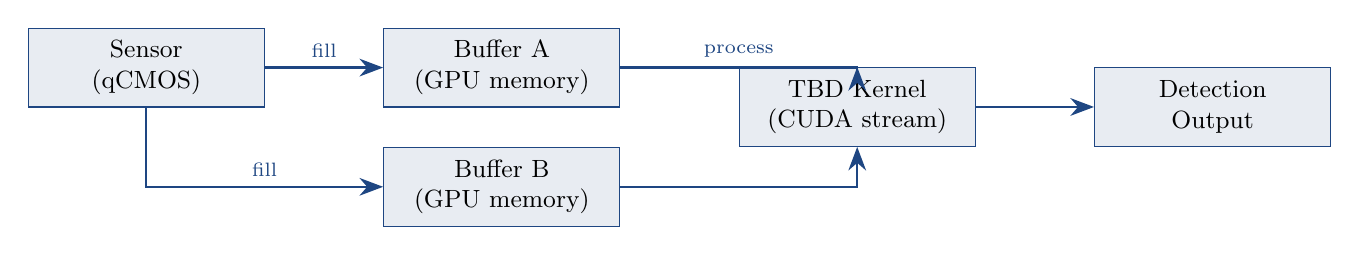
\begin{tikzpicture}[
    node distance=1.5cm,
    block/.style={rectangle, draw=zetablue, fill=zetablue!10,
        minimum width=3cm, minimum height=1cm, align=center,
        font=\small},
    arrow/.style={-{Stealth[length=3mm]}, thick, zetablue}
]
    \node[block] (sensor) {Sensor\\(qCMOS)};
    \node[block, right=1.5cm of sensor] (bufA) {Buffer A\\(GPU memory)};
    \node[block, below=0.5cm of bufA] (bufB) {Buffer B\\(GPU memory)};
    \node[block, right=1.5cm of bufA, yshift=-0.5cm] (kernel) {TBD Kernel\\(CUDA stream)};
    \node[block, right=1.5cm of kernel] (output) {Detection\\Output};

    \draw[arrow] (sensor) -- (bufA) node[midway, above, font=\scriptsize] {fill};
    \draw[arrow] (sensor) |- (bufB) node[near end, above, font=\scriptsize] {fill};
    \draw[arrow] (bufA) -| (kernel) node[near start, above, font=\scriptsize] {process};
    \draw[arrow] (bufB) -| (kernel);
    \draw[arrow] (kernel) -- (output);
\end{tikzpicture}
\end{center}

\begin{itemize}[leftmargin=2em]
    \item \textbf{Buffer A} receives frames while \textbf{Buffer B}
    is being processed by the TBD kernel (and vice versa)
    \item Use CUDA streams to overlap data ingest (CPU$\to$GPU copy or
    DMA from sensor) with kernel execution
    \item On Orin's unified memory, the ``copy'' may be a simple pointer
    swap if the sensor driver writes directly to managed memory
\end{itemize}

\subsubsection{Day 34--35: Preprocessing integration}

The raw sensor frames require preprocessing before TBD:
\begin{enumerate}[leftmargin=2em]
    \item \textbf{Dark frame subtraction:} $I_t \gets I_t - D$ where $D$
    is a pre-computed dark frame. This is a trivial element-wise CUDA
    kernel, but it must run in the same stream as the TBD kernel to avoid
    synchronization stalls.
    \item \textbf{Cosmic ray rejection:} Flag pixels exceeding a threshold
    (e.g., $> 5\sigma$) as invalid. Replace with local median or
    background estimate. This must be a separate kernel preceding TBD.
    \item \textbf{Star subtraction:} Remove known star signals using a
    catalog-based model. This requires catalog lookup and PSF-matched
    subtraction. Implement as a kernel or defer to a separate module
    depending on complexity.
\end{enumerate}

\noindent All preprocessing kernels should be fused where possible (e.g.,
dark subtraction + cosmic ray flagging in a single kernel pass) to
minimize memory traffic.

\subsection{Week 8: Thermal Validation and Documentation}

\subsubsection{Day 36--37: Sustained thermal testing}

\begin{itemize}[leftmargin=2em]
    \item Configure the Orin in its target power mode:
\begin{lstlisting}[style=bashstyle]
# Set power mode (example: 50W for space-sim conditions)
sudo nvpmodel -m 0         # Max performance (60W)
sudo nvpmodel -m 3         # 30W mode (closer to space thermal)
sudo jetson_clocks         # Lock clocks for reproducible measurements
\end{lstlisting}

    \item Run the full-scale benchmark continuously for 30+ minutes:
    \begin{itemize}
        \item Monitor GPU temperature:
            \texttt{tegrastats --interval 1000}
        \item Record throughput over time
        \item Identify if/when thermal throttling occurs
        \item Determine the \textbf{sustained} throughput (steady-state
            after thermal equilibrium) vs.\ the burst throughput
            (first 1--2 minutes)
    \end{itemize}

    \item The sustained throughput number is the one that matters for
    DARPA milestone reporting. Peak burst numbers are misleading for
    continuous operational scenarios.
\end{itemize}

\subsubsection{Day 38: Power profiling}

\begin{itemize}[leftmargin=2em]
    \item Measure actual power draw during kernel execution:
\begin{lstlisting}[style=bashstyle]
# Read power sensors on Orin
cat /sys/bus/i2c/drivers/ina3221/*/hwmon/hwmon*/power*_input
\end{lstlisting}

    \item Compute the energy efficiency metric:
    \begin{equation}
        \eta = \frac{\text{trajectories evaluated}}{\text{joules consumed}}
        \quad [\text{trajectories}/\text{J}]
    \end{equation}

    \item Compare across power modes. The optimal operating point
    may not be the highest-performance mode if the
    trajectories-per-joule efficiency peaks at a lower clock.
\end{itemize}

\subsubsection{Day 39--40: Documentation and delivery package}

Produce the following documentation for DARPA milestone delivery and
internal use:

\begin{enumerate}[leftmargin=2em]
    \item \textbf{Technical report:} Architecture description, optimization
    decisions and rationale, performance results on Orin, comparison to
    desktop GPU, scaling analysis.

    \item \textbf{Build and deployment guide:} Step-by-step instructions
    to compile and run on a fresh Orin developer kit. Include JetPack
    version requirements, build flags, and test procedures.

    \item \textbf{Performance datasheet:} One-page summary suitable for
    inclusion in DARPA milestone reports:
    \begin{itemize}
        \item Throughput (trajectories/second, pixels/second)
        \item Latency (wall-clock time for full-scale search)
        \item Power draw (watts, joules per search)
        \item Sustained vs.\ burst performance
    \end{itemize}

    \item \textbf{Validation report:} Detection results on all test
    datasets, including false alarm rate characterization, detection
    probability at varying SNR levels, and comparison to Python reference.

    \item \textbf{Source code:} Clean, documented, version-controlled
    repository with build system, test suite, and CI configuration.
\end{enumerate}

\begin{milestonebox}[Milestone 4 --- End of Week 8]
\textbf{Deliverables:}
\begin{enumerate}[leftmargin=2em]
    \item Complete TBD pipeline running on Orin: frame ingest $\to$
    preprocessing $\to$ TBD search $\to$ detection output
    \item Sustained thermal performance characterized
    \item Power efficiency measured across operating modes
    \item Full documentation package for DARPA milestone delivery
    \item Clean source repository with build system and test suite
\end{enumerate}
\textbf{Success criterion:} End-to-end pipeline runs correctly on Orin
under sustained thermal load. Documentation sufficient for DARPA review.
\end{milestonebox}

% ==============================================================
\section{Schedule Summary}
% ==============================================================

\begin{center}
\begin{ganttchart}[
    hgrid,
    vgrid={*{4}{draw=gray!30}},
    x unit=0.55cm,
    y unit chart=0.8cm,
    title height=1,
    title label font=\small\bfseries,
    bar height=0.5,
    bar label font=\small,
    milestone label font=\small\bfseries,
    group label font=\small\bfseries,
    bar/.append style={fill=zetablue!50, draw=zetablue},
    milestone/.append style={fill=milestone, draw=milestone!80!black},
]{1}{40}
    \gantttitle{Week 1}{5}
    \gantttitle{Week 2}{5}
    \gantttitle{Week 3}{5}
    \gantttitle{Week 4}{5}
    \gantttitle{Week 5}{5}
    \gantttitle{Week 6}{5}
    \gantttitle{Week 7}{5}
    \gantttitle{Week 8}{5} \\

    \ganttgroup[group/.append style={fill=phase1!30, draw=phase1}]
        {Phase 1: Bring-up}{1}{10} \\
    \ganttbar[bar/.append style={fill=phase1!50, draw=phase1}]
        {Environment + port}{1}{4} \\
    \ganttbar[bar/.append style={fill=phase1!50, draw=phase1}]
        {Validation framework}{5}{5} \\
    \ganttbar[bar/.append style={fill=phase1!50, draw=phase1}]
        {Profiling + analysis}{6}{10} \\
    \ganttmilestone{M1: Baseline}{10} \\

    \ganttgroup[group/.append style={fill=phase2!30, draw=phase2}]
        {Phase 2: Memory}{11}{20} \\
    \ganttbar[bar/.append style={fill=phase2!50, draw=phase2}]
        {Unified memory strategy}{11}{14} \\
    \ganttbar[bar/.append style={fill=phase2!50, draw=phase2}]
        {Prefetch + advise}{13}{15} \\
    \ganttbar[bar/.append style={fill=phase2!50, draw=phase2}]
        {L2 cache tuning}{16}{20} \\
    \ganttmilestone{M2: Memory opt.}{20} \\

    \ganttgroup[group/.append style={fill=phase3!30, draw=phase3}]
        {Phase 3: Kernel}{21}{30} \\
    \ganttbar[bar/.append style={fill=phase3!50, draw=phase3}]
        {Occupancy + block tuning}{21}{22} \\
    \ganttbar[bar/.append style={fill=phase3!50, draw=phase3}]
        {Early rejection}{23}{25} \\
    \ganttbar[bar/.append style={fill=phase3!50, draw=phase3}]
        {FP16 + warp reduction}{26}{30} \\
    \ganttmilestone{M3: Kernel opt.}{30} \\

    \ganttgroup[group/.append style={fill=phase4!30, draw=phase4}]
        {Phase 4: Integration}{31}{40} \\
    \ganttbar[bar/.append style={fill=phase4!50, draw=phase4}]
        {Pipeline integration}{31}{35} \\
    \ganttbar[bar/.append style={fill=phase4!50, draw=phase4}]
        {Thermal + power}{36}{38} \\
    \ganttbar[bar/.append style={fill=phase4!50, draw=phase4}]
        {Documentation}{39}{40} \\
    \ganttmilestone{M4: Delivery}{40}
\end{ganttchart}
\end{center}

% ==============================================================
\section{Risk Register}
% ==============================================================

\begin{table}[h]
\centering
\caption{Key risks and mitigations.}
\begin{tabular}{@{}p{3.2cm}cp{4cm}p{4.5cm}@{}}
\toprule
\textbf{Risk} & \textbf{Likelihood} & \textbf{Impact} & \textbf{Mitigation} \\
\midrule
Orin devkit hardware delay &
    Medium &
    Blocks all work until hardware arrives &
    Begin Phase 1 using Jetson Orin NX
    (pin-compatible, lower performance) or
    NVIDIA's cloud Jetson instances. \\
\addlinespace
Thermal throttling worse than expected &
    Medium &
    Sustained throughput $50$--$70\%$ of burst &
    Characterize early in Week 2.
    Adjust power mode and kernel duty cycle.
    Consider active cooling modifications. \\
\addlinespace
FP16 precision insufficient &
    Low &
    Detection results change vs.\ FP32 reference &
    Maintain FP32 fallback path.
    Validate FP16 at each SNR level.
    Use FP16 storage with FP32 accumulation
    (not pure FP16 compute). \\
\addlinespace
Unified memory performance pathological &
    Low &
    Page fault storms degrade bandwidth by
    $10\times$+ &
    Explicit prefetch on Day 1.
    Fall back to \texttt{cudaMalloc} with
    explicit copies if needed. \\
\addlinespace
Algorithm spec changes during 8 weeks &
    Medium &
    Rework required; schedule slips &
    Freeze algorithm spec before engineer
    starts. Changes queued for Phase 5 (post
    initial delivery). \\
\addlinespace
Engineer unfamiliar with Jetson platform &
    Medium &
    Weeks 1--2 take longer than planned &
    Budget 2 full weeks for bring-up.
    Provide Aethero BSP documentation on
    Day 1. Accept that this is the ramp-up
    cost. \\
\bottomrule
\end{tabular}
\end{table}

% ==============================================================
\section{Expected Outcome}
% ==============================================================

At the end of 8 weeks, the following performance envelope is expected for
the brute-force TBD kernel on the NVIDIA Jetson AGX Orin 64\,GB:

\begin{table}[h]
\centering
\caption{Projected performance at end of Week 8.}
\begin{tabular}{@{}lrr@{}}
\toprule
\textbf{Metric} & \textbf{Week 2 Baseline} & \textbf{Week 8 Target} \\
\midrule
Full-scale search time (burst)    & 10--30 min  & 2--5 min \\
Full-scale search time (sustained)& 15--40 min  & 3--8 min \\
Power draw                        & 60\,W (max) & 30--50\,W (tuned) \\
Energy per search                 & $\sim$50\,kJ & $\sim$10\,kJ \\
Memory footprint                  & 12\,GB (FP32) & 6\,GB (FP16) \\
\bottomrule
\end{tabular}
\end{table}

\begin{warnbox}[Important Context]
These numbers are for the \textbf{brute-force} algorithm at full
operational scale ($10\,\text{MP} \times 20\text{K velocities} \times
300\,\text{frames}$). The brute-force kernel is the correctness baseline,
not the operational target. The temporal-velocity pyramid and other
algorithmic accelerations (developed separately by the algorithm lead)
provide $100$--$1000\times$ additional reduction, bringing the operational
system into the real-time regime. The GPU engineer's optimized brute-force
kernel serves as:

\begin{enumerate}[leftmargin=2em]
    \item The correctness reference against which all accelerated
    algorithms are validated
    \item The inner-loop kernel that the accelerated algorithms invoke
    on reduced search spaces
    \item The worst-case fallback for regions where acceleration
    assumptions break down
\end{enumerate}
\end{warnbox}

\vfill
\begin{center}
\rule{0.5\textwidth}{0.4pt}\\[0.5em]
{\small\textcolor{gray}{%
    Zetascope, Inc.\ --- Internal Engineering Document\\
    Do not distribute outside the organization.
}}
\end{center}

\end{document}
